\section{Introduction}

\begin{figure}[H]
\centering
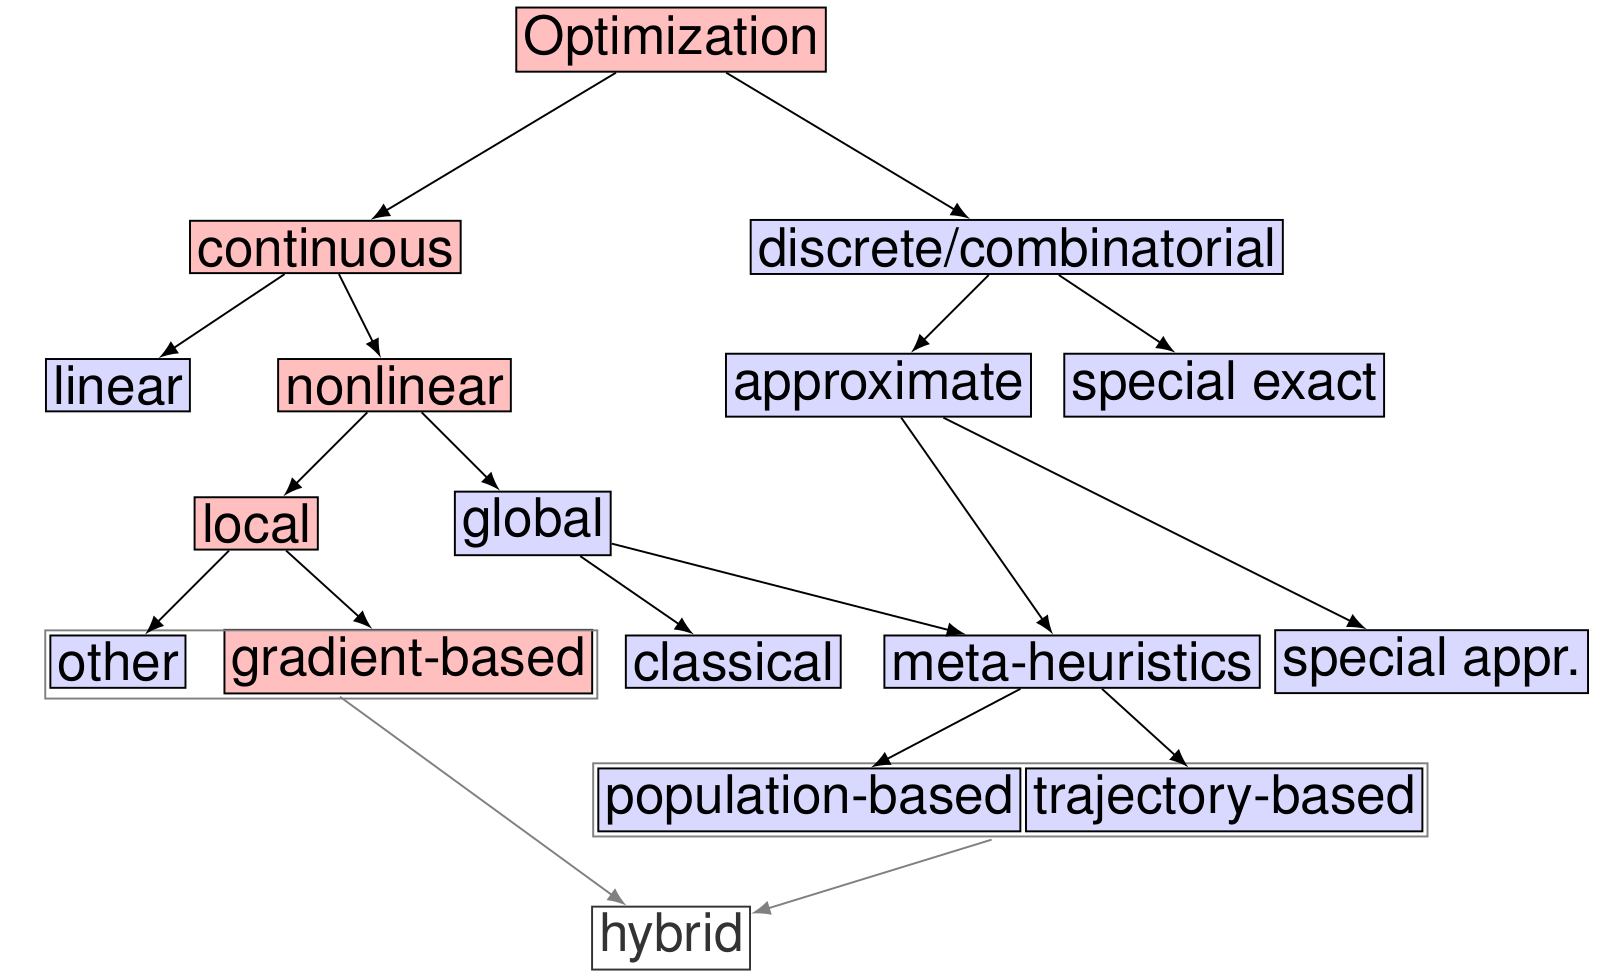
\includegraphics[width=0.8\textwidth]{figures/overview.png}
\caption{Optimization Overview}
\end{figure}

There are two fundamental types of Optimization
\begin{itemize}
    \item Continuous Optimization
    \begin{itemize}
        \item \textbf{Infinitely} many solutions, represented by continuous variables
        \item Main body of this theory is the \textbf{local optimization}
        \item Usually based on differential information
        \item E.g. using the gradient (1st derivative), which points in the direction of maximal function increase ("steepest ascent")
    \end{itemize}
    \item Discrete Optimization
    \begin{itemize}
        \item Only \textbf{finitely} many solutions, represented by integer variables
        \item Possibility of solving real-world problems
        \item Goal is to solve a specific problem in a reasonable time with a "good" algorithm
    \end{itemize}
\end{itemize}

\subsection{Complexity Theory}

Die Komplexitäts-Theorie beschreibt mit Hilfe der Zeit, die ein Algorithmus benötigt, um ein spezifisches Problem zu lösen, die Effektivität dieses Algorithmus.

\begin{itemize}
    \item Runtime depends on the size of the problem
    \item Best complexity is a linear growth of the runtime
    \item Size of the problem is somehow the number of bits for the parameters
    \item To make it HW \& SW independent, we focus on elementary operations in the code (e.g. addition, substraction, ...)
    \item We go for the most difficult instance of a given size n $\Rightarrow$ Worst Case
    \item Big O-Notation, $O(g(n))$, Big O of g.
    \item An algorithm is good, if his runtime is polynomial
    \item An algorithm is bad, if his runtime is exponential
\end{itemize}

\clearpage